

\begin{table*}
\centering
\small
\caption{\textcolor{red}{Question marks indicate fields that need to be completed. This list needs to be checked carefully.} List of velocity models currently supported by the UCVM platform.}
\begin{tabular}[]{lllllp{1.25in}}
%\hline
\\
Model Name         & Region                & String Label & Installation & Coverage Coordinates & References \\
\hline
SCEC CVM-H         & Southern California   &   cvmh        &  Automated   & ?         & \citet{Plesch_2011_SCEC}     \newline
                                                                                        \citet{CVM-H_Manual}         \newline
                                                                                        ?                            \\
SCEC CVM-S         & Southern California   &   cvms        &  Automated   & ?         & \citet{Magistrale_1996_BSSA} \newline
                                                                                        \citet{Magistrale_2000_BSSA} \newline
                                                                                        \citet{Kohler_2003_BSSA}     \\
SCEC CVM-S4.26     & Southern California   &   ?           &  Automated   & ?         & ?                            \\
Hadley-Kanamori 1D & ?                     &   1d          &  Automated   & ?         & ?                            \\
Carl Tape SoCal    & Southern California   &   tape        &  Manual      & ?         & ?                            \\
Broadband 1D       & Whittier Narrows      &   ?           &  Automated   & ?         & ?                            \\
Graves             & Cape Mendocino        &   cmrg        &  Manual      & ?         & ?                            \\
USGS CenCalVM      & Central California    &   cencal      &  Automated   & ?         & \citet{Brocher_2005_Tech}    \newline
                                                                                        \citet{Brocher_2006_Proc}    \\
SCEC CVM-NCI       & ?                     &   cvmnci      &  Manual      & ?         & ?                            \\
Lin-Thurber        & California Statewide  &   lt          &  Manual      & ?         & ?                            \\
USGS WFCVM         & Wasatch Front, Utah   &   wfcvm       &  Manual      & ?         & \citet{Magistrale_2006_Tech} \\
\hline
\end{tabular}
\label{tab:cvms}
\end{table*}





\begin{figure*}[ht!]
	\centering
	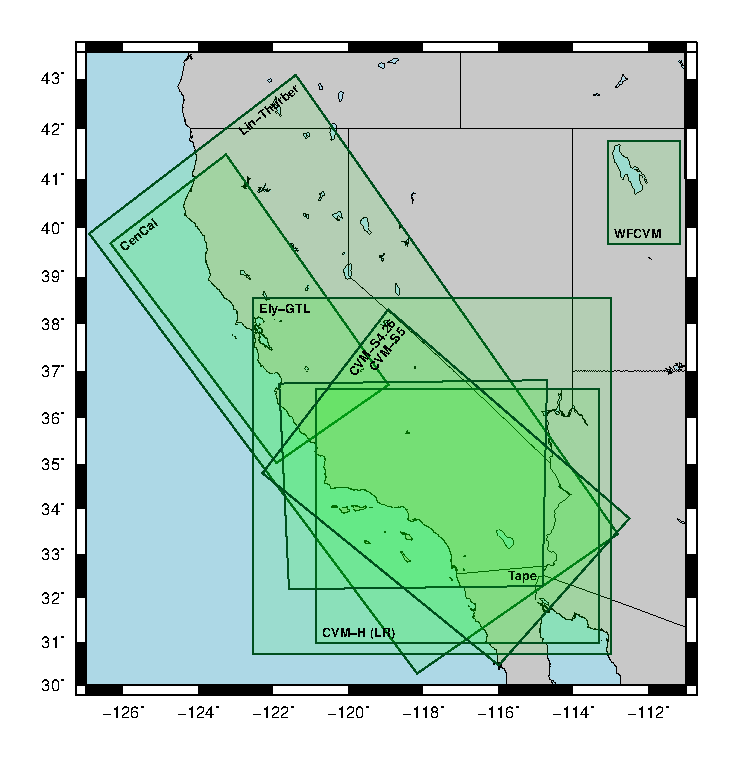
\includegraphics
		[width=0.7\textwidth]
		{figures/pdf/covered-areas}
	\caption{Surface horizontal projection of the areas covered by the various velocity models supported by the UCVM platform. See Table \ref{tab:cvms} for additional information and references.}
	\label{fig:cvms}
\end{figure*}


\section{Supported Velocity Models and Datasets}
\label{sec:cvms}

Velocity models vary considerably in terms of area of coverage, depth extent, composition, and resolution. The UCVM framework is flexible in its support for such variability and has been designed to integrate different velocity models, as well as to interact with their individual features seamlessly. UCVM has built-in support for a number of standard CVMs, which the platform utilities identify through corresponding string labels. Table \ref{tab:cvms} lists the models currently supported in the UCVM framework and provides additional details and references, along with their string labels. While all these models are supported by UCVM, only a selection of them are included in the automated installation package, as indicated in Table \ref{tab:cvms}. The remaining ones need to be installed manually before they can be accessed through the platform. Additional details are given in the documentation provided in Table \ref{tab:manuals} and in Section \ref{sec:easy.install}. Figure \ref{fig:cvms} shows a map with the coverage areas of various CVMs.

Velocity models need to be enabled at installation time. UCVM is distributed with an easy installation method which runs a Python script (\texttt{ucvm\_setup.py}) that prompts the user about which of the automated models are to be installed (see Section \ref{sec:easy.install}). If the user wants to enable other velocity models at a later time, the framework must be recompiled in order to enable the desired additional models. Advanced users can also customize the installation to support other models, including user-defined velocity models, which can be added in the form of an \textit{etree} \citep{Tu_2003_Tech} database or as a \textit{patch} (rasterized) model. These advanced features and other options mentioned here are described in greater detail in the UCVM Advanced User guide (see Table \ref{tab:manuals}), and are controlled at run-time through a configuration file read by UCVM which identifies the model(s) to be queried and the different alternative features.

In addition to the standard velocity models, UCVM includes two geotechnical layer (GTL) models, also listed in Table \ref{tab:cvms}. These models are intended to supplement (replace) the near-surface information in the original velocity models for a smoother transition from the softer near-surface soil deposits to the stiffer bedrock basement. The first of the two GTL models implements a \vsthirty-based interpolation from the free surface down to a given depth $z$, following \citet{Ely_2010_AGU}. The second GTL model is a generic one-dimensional (1D) model identical to the 1D crustal model. Two interpolation schemes can be used to smooth GTL material properties with the underlying crustal model material properties: a linear interpolation, or the interpolation relationship used by \citet{Ely_2010_AGU}. As in the case of the CVMs, the GTLs and the interpolation schemes are identified with string labels, \texttt{elygtl} and \texttt{1dgtl} for the \vsthirty-based and the 1D models, respectively. Similarly, the interpolation schemes are identified with the labels \texttt{ely} and \texttt{linear}. Note that the Ely GTL and interpolation models are used in the CVM-H model by default, with a reference depth of $z=350$~m. This option can be turned on or off for CVM-H by setting the model flag \texttt{USE\_GTL} \texttt{=} \texttt{true/false} in the configuration file.

To support the \vsthirty-based GTL model, UCVM has two built-in standard maps for California at 1 arcsec resolution (following USGS NED standards). These maps contain elevation data and \vsthirty{} data for the region. Using this information, \vsthirty{} values are assigned following one of two possible options. Option one implements the procedure by \citet{Wills_2006_BSSA} and \citet{Wald_2007_BSSA}. Option two follows \citet{Yong_2012_BSSA}. These options are identified by the string labels \texttt{ucvm}, which is the default option, and \texttt{yong}, respectively. These maps are stored as etree databases, and their details are included in Table \ref{tab:cvms} and Figure \ref{fig:cvms}.

The CVM-H model also provides an optional background 1D velocity structure supported by UCVM. This option allows queries at points outside and below the domain covered by the standard version of the model. While this option is inactive by default, it can be controlled manually by setting the model flag \texttt{USE\_1D\_BKG} \texttt{=} \texttt{true}. Other models can make use of this background structure by including the 1D model in the list of query models; that is, in the models sequence used to compose the meta-model. We refer to this process as tiling and explain its implementation in Section \ref{sec:querying}.

